\subsection{MAXIMAL TORI}

Let G be a Lie group. A torus of G is a closed subgroup that is a torus (§1, no. 2), in other words any commutative connected compact subgroup. The maximal elements of the set of tori of G, ordered by inclusion, are called the maximal tori of G.

THEOREM 2. Let G be a connected compact Lie group.

\begin{enumerate}
\def\labelenumi{\alph{enumi})}
\item
  The Lie algebras of the maximal tori of \(\mathbf{G}\) are the Cartan subalgebras of \(\mathrm{L}(\mathrm{G})\) .
\item
  Let \(\mathrm{T}_1\) and \(\mathrm{T}_2\) be two maximal tori of \(\mathbf{G}\) . There exists \(g \in \mathbf{G}\) such that \(\mathrm{T}_2 = g\mathrm{T}_1g^{-1}\) .
\item
  G is the union of its maximal tori.
\end{enumerate}

Let t be a Cartan subalgebra of L(G); the integral subgroup of G whose Lie algebra is t is closed (Chap. VII, §2, no. 1, Cor. 4 of Prop. 4) and commutative (Th. 1), and hence is a torus of G. If T is a maximal torus of G, its Lie algebra is commutative, hence is contained in a Cartan subalgebra of L(G) (Th. 1). It follows that the maximal tori of G are exactly the integral subgroups of G associated to the Cartan subalgebras of L(G), hence a). Assertion b) follows from Th. 1, since the canonical homomorphism G → Int(L(G)) is surjective (Chap. III, §6, no. 4, Cor. 4 of Prop. 10).

Denote by X the union of the maximal tori of G, and let T be a maximal torus of G. The continuous map \((g,t)\mapsto gtg^{-1}\) from \(G\times T\) to G has image X, which is therefore closed in G; thus, to prove c), it suffices to prove that X is open in G; since X is invariant under inner automorphisms, it suffices to show that, for all \(a \in \mathrm{T}\) , \(\mathrm{X}\) is a neighbourhood of \(a\) . We argue by induction on the dimension of \(\mathrm{G}\) and distinguish two cases:

\begin{enumerate}
\def\labelenumi{\arabic{enumi})}
\item
  a is not central in G. Let H be the identity component of the centralizer of a in G; this is a connected compact subgroup of G distinct from G, which contains T, and hence a. Since Ad a is semi-simple ( \(\S1\) , no. 1), the Lie algebra of H is the nilspace of Ad a - 1; it now follows from Chap. VII, \(\S4\) , no. 2, Prop. 4, that the union Y of the conjugates of H is a neighbourhood of a. By the induction hypothesis, \(H \subset X\) , and hence \(Y \subset X\) ; thus, X is a neighbourhood of a.
\item
  a is central in G. It suffices to prove that \(a \exp x\) belongs to X for all x in L(G). Now every element x of L(G) belongs to a Cartan subalgebra of G (Th. 1); the corresponding integral subgroup T' contains \(\exp x\) ; since it is conjugate to T, it contains a and hence \(a \exp x\) , as required.
\end{enumerate}

COROLLARY 1. a) The exponential map of \(\mathbf{G}\) is surjective.

\begin{enumerate}
\def\labelenumi{\alph{enumi})}
\setcounter{enumi}{1}
\tightlist
\item
  For all \(n \geq 1\) , the map \(g \mapsto g^n\) from \(\mathbf{G}\) to itself is surjective.
\end{enumerate}

Indeed, \(\exp(\mathrm{L}(\mathrm{G}))\) contains all the maximal tori of G, hence a). Assertion

\begin{enumerate}
\def\labelenumi{\alph{enumi})}
\setcounter{enumi}{1}
\tightlist
\item
  follows from the formula \((\exp x)^n = \exp nx\) for \(x\) in \(\mathrm{L}(\mathrm{G})\) .
\end{enumerate}

Remark 1. There exists a compact subset \(\mathrm{K}\) of \(\mathrm{L}(\mathrm{G})\) such that \(\exp_{\mathrm{G}}(\mathrm{K}) = \mathrm{G}\) . Indeed, if \(\mathrm{T}\) is a maximal torus of \(\mathrm{G}\) , there exists a compact subset \(\mathrm{C} \subset \mathrm{L}(\mathrm{T})\) such that \(\exp_{\mathrm{T}}(\mathrm{C}) = \mathrm{T}\) ; it suffices to take \(\mathrm{K} = \bigcup_{g \in \mathrm{G}} (\operatorname{Ad} g)(\mathrm{C})\) .

COROLLARY 2. The intersection of the maximal tori of G is the centre of G.

Let x be an element of the centre of G; by Th. 2 c), there exists a maximal torus T of G containing x; then x belongs to all the conjugates of T, hence to all the maximal tori of G. Conversely, if x belongs to all the maximal tori of G, it commutes with every element of G by Th. 2 c).

COROLLARY 3. Let \(g \in \mathbf{G}\) , and let \(\mathbf{C}\) be its centralizer. Then \(g\) belongs to \(\mathrm{C}_0\) ; the group \(\mathrm{C}_0\) is the union of the maximal tori of \(\mathbf{G}\) containing \(g\) .

There exists a maximal torus T of G containing g (Th. 2 c)), and hence contained in \(C_{0}\) . Moreover, the group \(C_{0}\) is a connected compact Lie group, and hence the union of its maximal tori (Th. 2 c)); these all contain g (Cor. 2), hence are exactly the maximal tori of G containing g.

COROLLARY 4. Let \(g \in G\) . If \(g\) is regular (Chap. VII, §4, no. 2, Def. 2), it belongs to a unique maximal torus, which is the identity component of its centralizer. Otherwise, it belongs to infinitely-many maximal tori.

Since Ad g is semi-simple, the dimension of the nilspace of Ad g-1 is also that of the centralizer C of g. By loc. cit., Prop. 8, and Th. 1, g is regular if and only if \(C_{0}\) is a maximal torus of G. The conclusion now follows from Cor. 3.

COROLLARY 5. a) Let S be a torus of G. The centralizer of S is connected; it is the union of the maximal tori of G containing S.

\begin{enumerate}
\def\labelenumi{\alph{enumi})}
\setcounter{enumi}{1}
\tightlist
\item
  Let \(\mathfrak{s}\) be a commutative subalgebra of \(\mathrm{L}(\mathrm{G})\) . The fixer of \(\mathfrak{s}\) in \(\mathrm{G}\) is connected; it is the union of the maximal tori of \(\mathrm{G}\) whose Lie algebras contain \(\mathfrak{s}\) .
\end{enumerate}

To prove \(a\) ), it suffices to prove that if an element \(g\) of G centralizes S, there exists a maximal torus of G containing S and \(g\) . Now, if C is the centralizer of \(g\) , we have \(g \in \mathrm{C}_0\) (Cor. 3) and \(\mathrm{S} \subset \mathrm{C}_0\) ; if T is a maximal torus of the connected compact Lie group \(\mathrm{C}_0\) containing S, we have \(g \in \mathrm{T}\) (Cor. 2), hence \(a\) ). Assertion \(b\) ) follows from \(a\) ) applied to the closure of the integral subgroup with Lie algebra \(\mathfrak{s}\) , in view of Chap. III, §9, no. 3, Prop. 9.

\pandocbounded{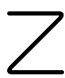
\includegraphics[keepaspectratio]{images/part002_b9f4d066.jpg}}

Remark 2. It follows from Cor. 5 that a maximal torus of G is a maximal commutative subgroup. The converse is not true: for example, in the group \(\mathbf{SO}(3,\mathbf{R})\) , the maximal tori are of dimension 1, and thus cannot contain the subgroup of diagonal matrices, which is isomorphic to \((\mathbf{Z}/2\mathbf{Z})^{2}\) . Moreover, if \(g \in \mathbf{SO}(3,\mathbf{R})\) is a non-scalar diagonal matrix, g is a regular element of \(\mathbf{SO}(3,\mathbf{R})\) whose centralizer is not connected (cf.~Cor. 4).

COROLLARY 6. The maximal tori of G are their own centralizers, and are the fixers of their Lie algebras.

Let T be a maximal torus of G and C its centralizer; since \(L(T)\) is a Cartan subalgebra of \(L(G)\) , we have \(L(T) = L(C)\) , hence C = T since C is connected (Cor. 5).

COROLLARY 7. Let T and T' be two maximal tori of G, A a subset of T and s an automorphism of G that takes A into T'. There exists \(g \in G\) such that \(s \circ (\operatorname{Int} g)\) takes T to T' and coincides with s on A.

Let C be the centralizer of A. Then T and \(s^{-1}(T')\) are two maximal tori of \(C_{0}\) ; every element g of \(C_{0}\) such that \((\operatorname{Int} g)(\mathrm{T}) = s^{-1}(\mathrm{T}')\) has the desired properties.

COROLLARY 8. Let H be a compact Lie group, T a maximal torus of H. Then \(\mathrm{H} = \mathrm{N}_{\mathrm{H}}(\mathrm{T}) \cdot \mathrm{H}_{0}\) , and the injection of \(\mathrm{N}_{\mathrm{H}}(\mathrm{T})\) into H induces an isomorphism from \(\mathrm{N}_{\mathrm{H}}(\mathrm{T}) / \mathrm{N}_{\mathrm{H}_{0}}(\mathrm{T})\) to \(H/H_{0}\) .

Let \(h \in H\) . Then \(h^{-1}Th\) is a maximal torus of \(H_0\) , hence (Th. 2) there exists \(g \in H_0\) such that \(hg \in N_H(T)\) ; thus \(h\) belongs to \(N_H(T).H_0\) , hence the first assertion. The second follows immediately.

Remarks. 3) Let G be a connected Lie group whose Lie algebra is compact. The Cartan subgroups of G are the integral subgroups whose Lie algebras are the Cartan subalgebras of L(G) (the Cartan subgroups of a connected compact group are thus its maximal tori). Theorem 2 and its corollaries remain valid for G, if we replace everywhere the expression ``maximal torus'' by ``Cartan subgroup''. This follows immediately from the fact that, in view of Prop. 5 of §1, no. 4, G is the direct product of a vector group V and a connected compact group K and that the Cartan subgroups of G are the products of V with the maximal tori of K. Moreover, note that it follows from Cor. 6 above that the Cartan subgroups of G can also be defined as the fixers of the Cartan subalgebras of L(G).

* 4) Part \(c\) of Theorem 2 can also be proved in the following way. Give G an invariant riemannian metric (§1, no. 3, Prop. 3). Then, for any element \(g\) of G, there exists a maximal geodesic passing through \(g\) and the identity element of G (Hopf-Rinow theorem), and it can be verified that the closure of such a geodesic is a subtorus of G. *

